\section*{Anhang}

\begin{table}[H]
  \centering
  \begin{tabular}{l c c}
    \hline
    \textbf{Arbeitspaket} & \textbf{Dauer} & \textbf{Gesamt} \\
    \hline
    Analyse                                              &                & \qty{5}{\hour} \\
    \quad Durchführung der IST-Analyse                   & \qty{2}{\hour}  &  \\
    \quad Ausarbeitung der SOLL-Analyse                  & \qty{3}{\hour}  &  \\
    Planung                                              &                & \qty{20}{\hour} \\
    \quad Evaluierung der Umsetzungsmöglichkeiten        & \qty{5}{\hour}  &  \\
    \quad Entwurf der Schnittstellenarchitektur          & \qty{7}{\hour}  &  \\
    \quad Kostenschätzung und Ressourcenplanung          & \qty{4}{\hour}  &  \\
    \quad Testplanung                                    & \qty{4}{\hour}  &  \\
    Realisierung                                         &                & \qty{40}{\hour} \\
    \quad Einrichtung des Projekts und Systemumgebung    & \qty{4}{\hour}  &  \\
    \quad Design der Schnittstelle und Architektur       & \qty{7}{\hour}  &  \\
    \quad Implementierung der Schnittstelle              & \qty{20}{\hour} &  \\
    \quad Durchführung von Tests und Fehlerbehebung      & \qty{5}{\hour}  &  \\
    \quad Anpassungen basierend auf Testergebnissen      & \qty{4}{\hour}  &  \\
    Abnahme                                              &                & \qty{2}{\hour} \\
    Projektdokumentation                                 &                & \qty{7}{\hour} \\
    Kundendokumentation                                  &                & \qty{4}{\hour} \\
    Pufferzeit                                           &                & \qty{2}{\hour} \\
    \hline
    \textbf{Gesamt} &  & \textbf{80 h} \\
    \hline
  \end{tabular}
  \caption{Detaillierte Zeitplanung}
  \label{tab:genaue-zeitplanung}
\end{table}

\begin{table}[H]
  \centering
  \begin{tabular}{l l}
    \hline
    \textbf{Hardware}   &  \\
    \hline
    Arbeitslaptop    & mit Anschlussmöglichkeiten an Strom \& Ethernet \\
    Büroarbeitsplatz mit zusätzlichen Geräten & Monitor, Maus und Tastatur\\
    Headset        & für Online Meetings \\
    \hline
    \textbf{Software}   &  \\
    \hline
    Arch Linux      & Betriebssystem \\
    Neovim         & Text-Editor \\
    Python        & Programmiersprache \\
    Git          & Versionsverwaltung \\
    GitLab        & Online-Plattform zum Speichern des Repositorys \\
    MetricQ        & Framework zum Zugriff auf die zu verarbeiten Daten \\
    pydantic      & Framework zum Validieren und lesen von u.\,a. JSONs \\
    Mermaid.js      & Tool zum Erstellen von Diagrammen \\
    Firefox        & zum Nachschlagen von Dokumentationen \\
    LaTeX        & Sprache zum Schreiben der Projektarbeit\\
    Overleaf      & Tool / Speicher für Latex-Dokumente\\
    \hline
    \textbf{Personal}   &  \\
    \hline
    Projektbetreuer    & Ansprechpartner für die gewünschten Funktionen \\
    Monitoring-Verantwortlicher  & Ansprechpartner für Probleme mit Checkmk \\
    Entwickler      & Umsetzung des Projekts / Autor \\
  \end{tabular}
  \caption{Verwendete Ressourcen}
  \label{tab:verwendete-ressourcen}
\end{table}

\begin{figure}[H]
  \centering
  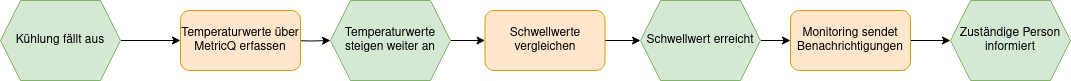
\includegraphics[width=\textwidth]{images/epk-cooling-fails.png}
  \caption{EPK Ausfall der Kühlung}
  \label{fig:epk-cooling-fails}
\end{figure}

\begin{figure}[H]
  \centering
  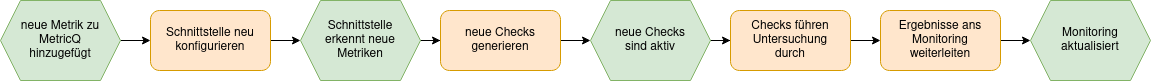
\includegraphics[width=\textwidth]{images/epk-structure-change.png}
  \caption{EPK Änderung der Struktur}
  \label{fig:epk-structure-changes}
\end{figure}

\begin{table}[H]
  \centering
  \begin{tabular}{l c c c}
    \hline
    \textbf{Eigenschaft} & \textbf{Gewichtung} & \textbf{C++} & \textbf{Python}\\
    \hline
    Standardaufgaben                    & 0.2   & 3   & 4 \\
    Erstellen von Testfällen            & 0.3   & 2   & 3 \\
    Programmiergeschwindigkeit          & 0.5   & 2   & 4 \\
    Performance                         & 0.1   & 4   & 2 \\
    Kompatibilität                      & 0.2   & 4   & 4 \\
    Verfügbarkeit von Bibliotheken      & 0.1   & 2   & 4 \\
    Wartbarkeit und Lesbarkeit          & 0.4   & 2   & 4 \\
    \hline
    \textbf{Gesamt}                     & 1.8   & 4.4 & 6.7 \\
    \hline
  \end{tabular}
  \caption{Entscheidungsmatrix: Vergleich von C++ und Python}
  \label{tab:entscheidungsmatrix}
\end{table}

\begin{figure}[H]
  \centering
  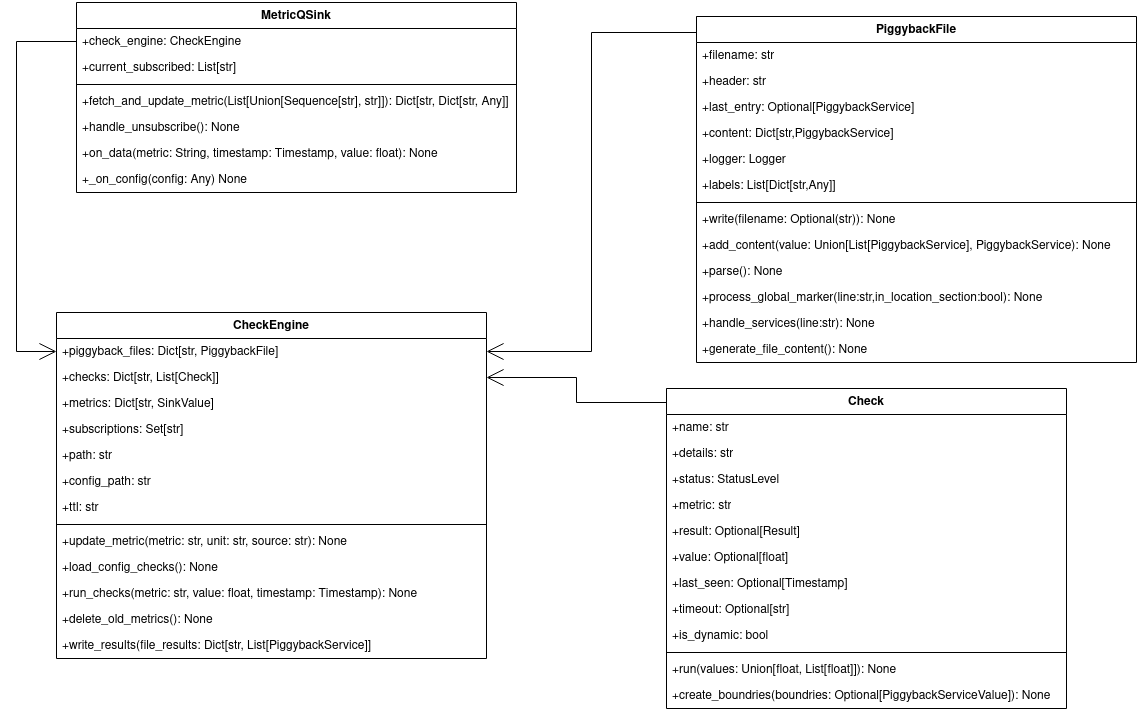
\includegraphics[width=\textwidth]{images/class-diagram.png}
  \caption{Klassendiagramm}
  \label{fig:class-diagram}
\end{figure}

\begin{lstlisting}[language=Python, caption=MetricQSink-Klasse, label=lst:metricq_sink]
class MetricQSink(metricq.DurableSink):
    """
    A MetricQ sink that processes incoming data points and checks them using CheckEngine.
    """

    def __init__(
        self, path: str, config_path: str, ttl: int, *args: Any, **kwargs: Any
    ):
    ..

    async def on_data(
        self, metric: str, timestamp: metricq.Timestamp, value: float
    ) -> None:
    ...

    @metricq.rpc_handler("config")
    async def _on_config(self, **config: Any):
          ...

    async def fetch_and_update_metrics(
        self, subscriptions: List[Union[Sequence[str], str]]
    ) -> Dict[str, Dict[str, Any]]:
        """
        Fetch metric data (with both historic data and metadata) based on subscriptions,
        and update the CheckEngine with the metric metadata.

        Returns:
            Dict[str, Dict[str, Any]]: The metric data for further processing.
        """
        ...

    async def handle_unsubscribe(self) -> None:
        """
        Handle unsubscribing from metrics that are no longer part of any active check.
        """
        ...
\end{lstlisting}

\begin{lstlisting}[language=Python, caption=CheckEngine-Klasse, label=lst:check_engine]
class Check:
    """
    A class used to perform a health check on a set of numerical values.
    """
    def set_result(self) -> None:
        """
        Build and set the check result based on the current evaluation.

        Creates a new Result instance with the check's name, current status, average value,
        and associated threshold boundaries. If the unit is not set, a default placeholder ("-")
        is used.
        """
        unit = self.__unit
        if not unit:
            unit = "-"

        if self.__value is None:
            unit = "-"

        self.__result = Result(
            name=self.__name,
            status=self.__status,
            value=PiggybackServiceValue(
                unit=unit,
                value=self.__value,
                warn=self.__warn,
                crit=self.__crit,
                min=self.__min,
                max=self.__max,
            ),
            details=self.__details,
        )
\end{lstlisting}

\begin{table}[H]
  \centering
  \begin{tabular}{l c c c}
    \hline
    \textbf{Projektphase} & \textbf{Geplante Zeit} & \textbf{Gebrauchte Zeit} & \textbf{Differenz}\\
    \hline
    Analyse                 & \qty{5}{\hour}  & \qty{5}{\hour}  & \qty{0}{\hour}\\
    Planung                 & \qty{20}{\hour} & \qty{20}{\hour} & \qty{0}{\hour} \\
    Realisierung            & \qty{40}{\hour} & \qty{42}{\hour} & + \qty{2}{\hour} (Pufferzeit) \\
    Abnahme                 & \qty{2}{\hour}  & \qty{2}{\hour}  & \qty{0}{\hour} \\
    Projektdokumentation    & \qty{7}{\hour}  & \qty{7}{\hour}  & \qty{0}{\hour} \\
    Kundendokumentation     & \qty{4}{\hour}  & \qty{4}{\hour}  & \qty{0}{\hour} \\
    Pufferzeit              & \qty{2}{\hour}  & \qty{2}{\hour}  & \qty{0}{\hour} \\
    \hline
    \textbf{Gesamt} & \textbf{80 h} & \textbf{80 h} & \textbf{0 h} \\
    \hline
  \end{tabular}
  \caption{Zeitvergleich}
  \label{tab:zeitvergleich}
\end{table}

\begin{lstlisting}[language=Bash, caption=Unit-Tests, label=lst:unit-test]
> pytest
================== test session starts ==================
platform linux -- Python 3.13.2, pytest-8.3.5, pluggy-1.5.0
rootdir: /home/flmr799e/GIT/work/GitLab/checkQ
configfile: pyproject.toml
collected 35 items

tests/piggyback/test_piggyback_file.py .....             [ 14%]
tests/piggyback/test_piggyback_service.py ....           [ 25%]
tests/piggyback/test_piggyback_service_value.py ......   [ 42%]
tests/piggyback/test_threshold.py ........               [ 65%]
tests/test_check.py ..........                           [ 94%]
tests/test_check_engine.py ..                            [100%]

================== 35 passed in 0.17s ==================

\end{lstlisting}

\begin{figure}[H]
  \centering
  
\includegraphics[width=\textwidth]{images/tbd.png}
  \caption{Weboberfläche}
  \label{fig:checkmk_check_uebersicht}
\end{figure}
